\section{Бинарный аддитивный e-индикатор.}
Определение\\
Бинарный аддитивный $e$-индикатор: $e(A, B)$ = минимальное $x$, такое что
множество ${a − (x, x,...,x) : a ∈A}$ доминирует каждое решение из $B$\\

\begin{figure}[!ht]
Этот индикатор работает на подмножествах множествах решений в отличие от просто бинарного индикатора, который работает на 2-ух решениях из всего множества
\begin{center}
    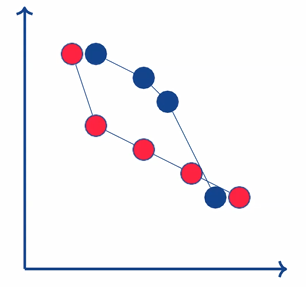
\includegraphics[width=0.3\linewidth]{images/e-indicator1.PNG}
    \caption{$e$-indicator first position}
    \label{fig:mpr}
    
\end{center}

\end{figure}

\begin{figure}[!ht]

\begin{center}
    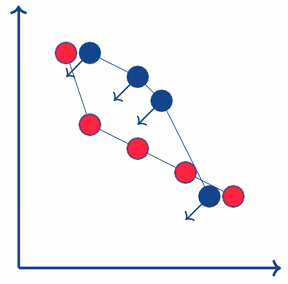
\includegraphics[width=0.3\linewidth]{images/e-indicator3.PNG}
    \caption{$e$-indicator second position}
    \label{fig:mpr}
    
\end{center}

\end{figure}

\begin{figure}[!ht]
Оптимальное решение - то, которое максимально близко к границе множества (одна из 2-ух синих точек в центре)
\begin{center}
    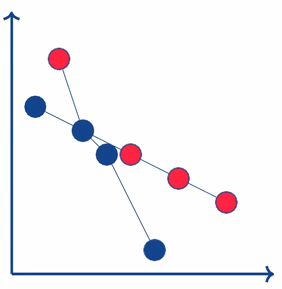
\includegraphics[width=0.3\linewidth]{images/e-indicator2.PNG}
    \caption{$e$-indicator third position}
    \label{fig:mpr}
    
\end{center}

\end{figure}

\newpage

Свойства\\
(+): O(N2K), вычисляется просто и относительно быстро\\
$O(min(NK\log_{N}^_{(K − 2)}$, $+ NK^2, N^2K))$ с 2016 года\\
(+): слабо, но коррелирует с отношением доминирования
$(A ≺ B → e(A,B) ≤ 0)$. Пример, когда $e$ = 0:
(−): не антисимметрично ($e(A,B)$ /= $−e(B,A))$ (данный индикатор не работает на обратных множествах, порядок множества важен!) ,
оба варианта могут быть положительными,
полный порядок отсутствует\\

Расширения\\
Унарный $e$-индикатор: $e(A) = ε(A,S)$ для фиксированного множества $S$\\
Мультипликативный $e$-индикатор: не вычитать $e$, а умножать на $e$
